\documentclass[12pt]{article}
 
\usepackage[margin=0.8in]{geometry}
\usepackage{amsmath}
\usepackage{amssymb}
\usepackage{graphicx}
\usepackage{tikz}
\usepackage{pgfplots}

\pgfplotsset{compat=1.18}

\title{Precalculus: Functions and Their Graphs}
\author{Ryan Lee}
\date{\today}

\begin{document}

\maketitle

\section{Lines in the Plane}

Lines are fundamental objects in precalculus and can be represented in various forms.

\subsection{Slope-Intercept Form}

The slope-intercept form of a line is $y = mx + b$, where:
\begin{itemize}
    \item $m$ is the slope (rate of change)
    \item $b$ is the y-intercept (where the line crosses the y-axis)
\end{itemize}

\subsection{Point-Slope Form}

The point-slope form is $y - y_1 = m(x - x_1)$, where $(x_1, y_1)$ is a point on the line and $m$ is the slope.

\subsection{Slope Formula}

For two points $(x_1, y_1)$ and $(x_2, y_2)$, the slope is:

\[m = \frac{y_2 - y_1}{x_2 - x_1}\]

\subsection{Example 1: Finding the Equation of a Line}

Find the equation of a line passing through points (1, 3) and (4, 9).

Solution:
1) Calculate the slope:
   $m = \frac{9 - 3}{4 - 1} = \frac{6}{3} = 2$
   
2) Use point-slope form with (1, 3):
   $y - 3 = 2(x - 1)$
   
3) Simplify to slope-intercept form:
   $y = 2x + 1$

\begin{center}
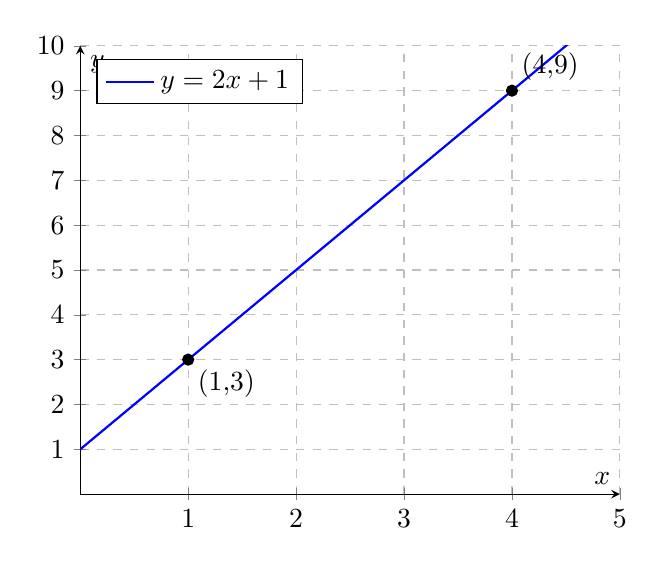
\begin{tikzpicture}
\begin{axis}[
    axis lines = middle,
    xlabel = $x$,
    ylabel = $y$,
    xmin = 0, xmax = 5,
    ymin = 0, ymax = 10,
    xtick = {1,2,3,4,5},
    ytick = {1,2,3,4,5,6,7,8,9,10},
    legend pos = north west,
    ymajorgrids = true,
    xmajorgrids = true,
    grid style = dashed,
]

\addplot[
    domain = 0:5,
    samples = 2,
    smooth,
    thick,
    blue,
]
{2*x + 1};
\addlegendentry{$y = 2x + 1$}

\addplot[only marks,mark=*] coordinates {(1,3) (4,9)};
\node[anchor=north west] at (axis cs: 1,3) {(1,3)};
\node[anchor=south west] at (axis cs: 4,9) {(4,9)};

\end{axis}
\end{tikzpicture}
\end{center}

\section{Functions}

A function is a rule that assigns each element of one set (domain) to exactly one element of another set (range).

\subsection{Key Concepts}

\begin{itemize}
    \item Domain: Set of all possible input values (x-values)
    \item Range: Set of all possible output values (y-values)
    \item Independent variable: Input variable (usually x)
    \item Dependent variable: Output variable (usually y)
\end{itemize}

\subsection{Function Notation}

We write $f(x) = y$ to denote a function $f$ that takes an input $x$ and produces an output $y$.

\subsection{Evaluating Functions}

To evaluate a function, substitute the given x-value into the function.

\subsection{Example 2: Evaluating a Function}

If $f(x) = x^2 - 3x + 2$, find $f(4)$ and $f(-1)$.

Solution:
For $f(4)$: 
$f(4) = (4)^2 - 3(4) + 2 = 16 - 12 + 2 = 6$

For $f(-1)$:
$f(-1) = (-1)^2 - 3(-1) + 2 = 1 + 3 + 2 = 6$

\subsection{Vertical Line Test}

A graph represents a function if and only if no vertical line intersects the graph more than once.

\begin{center}
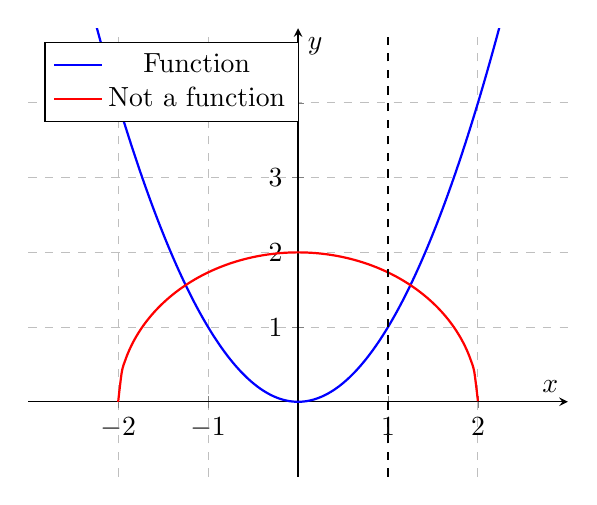
\begin{tikzpicture}
\begin{axis}[
    axis lines = middle,
    xlabel = $x$,
    ylabel = $y$,
    xmin = -3, xmax = 3,
    ymin = -1, ymax = 5,
    xtick = {-2,-1,0,1,2},
    ytick = {0,1,2,3,4},
    legend pos = north west,
    ymajorgrids = true,
    xmajorgrids = true,
    grid style = dashed,
]

\addplot[
    domain = -3:3,
    samples = 100,
    smooth,
    thick,
    blue,
]
{x^2};
\addlegendentry{Function}

\addplot[
    domain = -2:2,
    samples = 100,
    smooth,
    thick,
    red,
]
{sqrt(4-x^2)};
\addlegendentry{Not a function}

\draw[dashed] (1,-1) -- (1,5);
\node[anchor=north] at (1,-1) {Vertical line};

\end{axis}
\end{tikzpicture}
\end{center}

\section{Graphs of Functions}

The graph of a function is the set of all points $(x, y)$ where $y = f(x)$.

\subsection{Key Features of Graphs}

\begin{itemize}
    \item x-intercepts: Points where the graph crosses the x-axis $(f(x) = 0)$
    \item y-intercept: Point where the graph crosses the y-axis $(x = 0)$
    \item Increasing/Decreasing: Intervals where the function values increase or decrease
    \item Maximum/Minimum points: Highest and lowest points on the graph
\end{itemize}

\subsection{Example 3: Analyzing a Graph}

Consider the graph of $f(x) = x^3 - 3x^2 - 9x + 5$:

\begin{center}
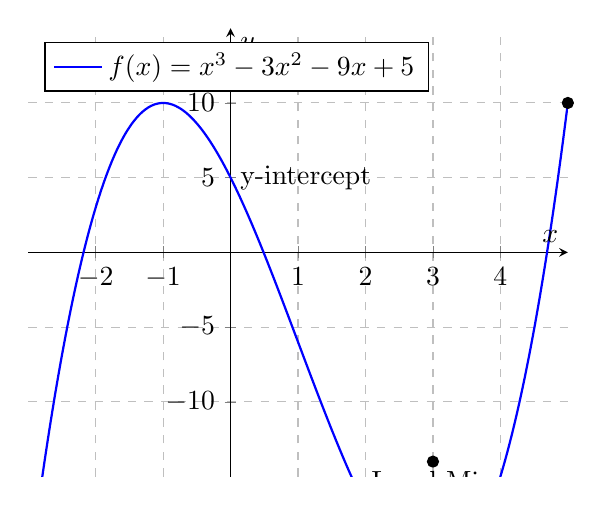
\begin{tikzpicture}
\begin{axis}[
    axis lines = middle,
    xlabel = $x$,
    ylabel = $y$,
    xmin = -3, xmax = 5,
    ymin = -15, ymax = 15,
    xtick = {-2,-1,0,1,2,3,4},
    ytick = {-10,-5,0,5,10},
    legend pos = north west,
    ymajorgrids = true,
    xmajorgrids = true,
    grid style = dashed,
]

\addplot[
    domain = -3:5,
    samples = 100,
    smooth,
    thick,
    blue,
]
{x^3 - 3*x^2 - 9*x + 5};
\addlegendentry{$f(x) = x^3 - 3x^2 - 9x + 5$}

\addplot[only marks,mark=*] coordinates {(-1,18) (3,-14) (5,10)};
\node[anchor=south] at (axis cs: -1,18) {Local Max};
\node[anchor=north] at (axis cs: 3,-14) {Local Min};
\node[anchor=west] at (axis cs: 0,5) {y-intercept};

\end{axis}
\end{tikzpicture}
\end{center}

Observations:
\begin{itemize}
    \item y-intercept: (0, 5)
    \item x-intercepts: approximately at x = -1.5, x = 1, and x = 3.5
    \item Local maximum at approximately (-1, 18)
    \item Local minimum at approximately (3, -14)
    \item Increasing on intervals (-∞, -1) and (3, ∞)
    \item Decreasing on interval (-1, 3)
\end{itemize}

\section{Transformations of Functions}

Transformations allow us to modify the graph of a function in predictable ways.

\subsection{Shifting Graphs}

\subsubsection{Vertical Shifts}

For a function $f(x)$:
\begin{itemize}
    \item $f(x) + k$ shifts the graph $k$ units up
    \item $f(x) - k$ shifts the graph $k$ units down
\end{itemize}

\subsubsection{Horizontal Shifts}

For a function $f(x)$:
\begin{itemize}
    \item $f(x - h)$ shifts the graph $h$ units right
    \item $f(x + h)$ shifts the graph $h$ units left
\end{itemize}

\subsection{Example 4: Shifting Graphs}

Consider the function $f(x) = x^2$. Graph $f(x)$, $f(x) + 2$, and $f(x - 1)$.

\begin{center}
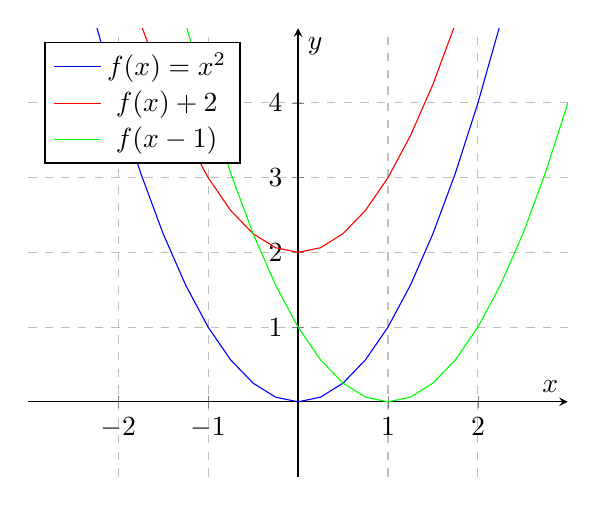
\begin{tikzpicture}
\begin{axis}[
    axis lines = middle,
    xlabel = $x$,
    ylabel = $y$,
    xmin = -3, xmax = 3,
    ymin = -1, ymax = 5,
    xtick = {-2,-1,0,1,2},
    ytick = {0,1,2,3,4},
    legend pos = north west,
    ymajorgrids = true,
    xmajorgrids = true,
    grid style = dashed,
]

\addplot[domain=-3:3, blue] {x^2};
\addlegendentry{$f(x) = x^2$}

\addplot[domain=-3:3, red] {x^2 + 2};
\addlegendentry{$f(x) + 2$}

\addplot[domain=-3:3, green] {(x-1)^2};
\addlegendentry{$f(x-1)$}

\end{axis}
\end{tikzpicture}
\end{center}

\subsection{Reflecting Graphs}

\begin{itemize}
    \item $-f(x)$ reflects the graph of $f(x)$ over the x-axis
    \item $f(-x)$ reflects the graph of $f(x)$ over the y-axis
\end{itemize}

\subsection{Example 5: Reflecting Graphs}

Graph $f(x) = |x|$, $-f(x)$, and $f(-x)$.

\begin{center}
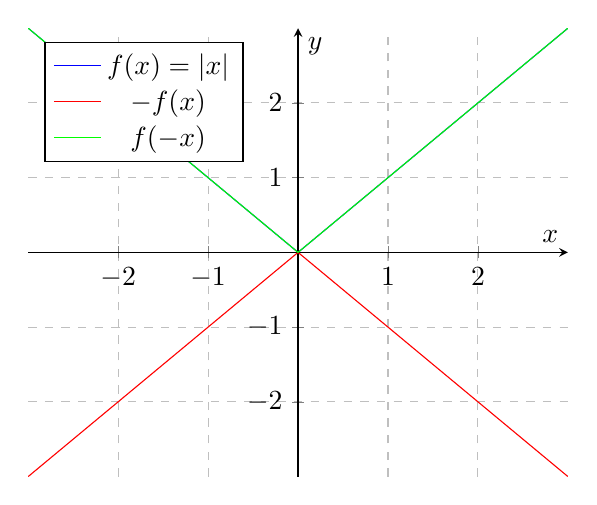
\begin{tikzpicture}
\begin{axis}[
    axis lines = middle,
    xlabel = $x$,
    ylabel = $y$,
    xmin = -3, xmax = 3,
    ymin = -3, ymax = 3,
    xtick = {-2,-1,0,1,2},
    ytick = {-2,-1,0,1,2},
    legend pos = north west,
    ymajorgrids = true,
    xmajorgrids = true,
    grid style = dashed,
]

\addplot[domain=-3:3, blue] {abs(x)};
\addlegendentry{$f(x) = |x|$}

\addplot[domain=-3:3, red] {-abs(x)};
\addlegendentry{$-f(x)$}

\addplot[domain=-3:3, green] {abs(-x)};
\addlegendentry{$f(-x)$}

\end{axis}
\end{tikzpicture}
\end{center}

\subsection{Stretching and Compressing Graphs}

For a constant $a > 0$:
\begin{itemize}
    \item $af(x)$ stretches the graph vertically by a factor of $a$ if $a > 1$, or compresses it if $0 < a < 1$
    \item $f(ax)$ compresses the graph horizontally by a factor of $a$ if $a > 1$, or stretches it if $0 < a < 1$
\end{itemize}

\subsection{Example 6: Stretching and Compressing}

Graph $f(x) = x^2$, $2f(x)$, and $f(2x)$.

\begin{center}
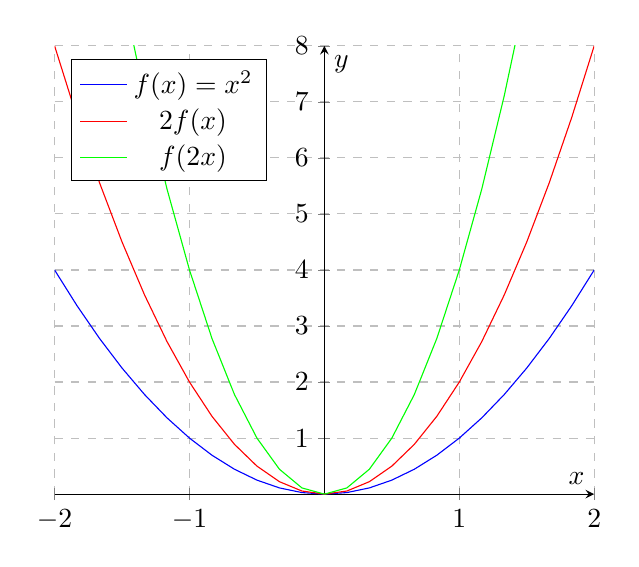
\begin{tikzpicture}
\begin{axis}[
    axis lines = middle,
    xlabel = $x$,
    ylabel = $y$,
    xmin = -2, xmax = 2,
    ymin = 0, ymax = 8,
    xtick = {-2,-1,0,1,2},
    ytick = {0,1,2,3,4,5,6,7,8},
    legend pos = north west,
    ymajorgrids = true,
    xmajorgrids = true,
    grid style = dashed,
]

\addplot[domain=-2:2, blue] {x^2};
\addlegendentry{$f(x) = x^2$}

\addplot[domain=-2:2, red] {2*x^2};
\addlegendentry{$2f(x)$}

\addplot[domain=-2:2, green] {(2*x)^2};
\addlegendentry{$f(2x)$}

\end{axis}
\end{tikzpicture}
\end{center}

\section{Combinations of Functions}

We can combine functions to create new functions using basic arithmetic operations.

\subsection{Sum and Difference}

For functions $f(x)$ and $g(x)$:
\begin{itemize}
    \item $(f + g)(x) = f(x) + g(x)$
    \item $(f - g)(x) = f(x) - g(x)$
\end{itemize}

\subsection{Product and Quotient}

For functions $f(x)$ and $g(x)$:
\begin{itemize}
    \item $(f \cdot g)(x) = f(x) \cdot g(x)$
    \item $(\frac{f}{g})(x) = \frac{f(x)}{g(x)}$, where $g(x) \neq 0$
\end{itemize}

\subsection{Composition}

The composition of $f$ and $g$ is denoted as $(f \circ g)(x) = f(g(x))$.

\subsection{Example 7: Function Combinations}

Let $f(x) = x^2$ and $g(x) = x + 1$. Find and evaluate at $x = 2$:
\begin{itemize}
    \item $(f + g)(x)$
    \item $(f \cdot g)(x)$
    \item $(f \circ g)(x)$
\end{itemize}

Solution:
\begin{itemize}
    \item $(f + g)(x) = x^2 + (x + 1)$
      $(f + g)(2) = 2^2 + (2 + 1) = 4 + 3 = 7$
    \item $(f \cdot g)(x) = x^2(x + 1)$
      $(f \cdot g)(2) = 2^2(2 + 1) = 4 \cdot 3 = 12$
    \item $(f \circ g)(x) = f(g(x)) = f(x + 1) = (x + 1)^2$
      $(f \circ g)(2) = (2 + 1)^2 = 3^2 = 9$
\end{itemize}

\subsection{Graphical Representation of Function Combinations}

Let's visualize the combinations of $f(x) = x^2$ and $g(x) = x + 1$.

\begin{center}
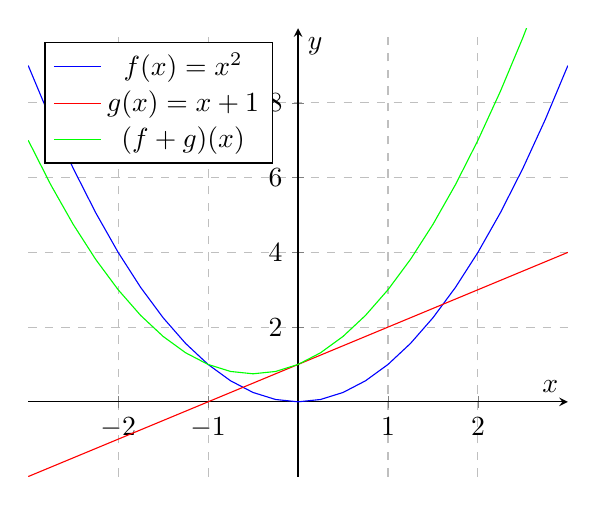
\begin{tikzpicture}
\begin{axis}[
    axis lines = middle,
    xlabel = $x$,
    ylabel = $y$,
    xmin = -3, xmax = 3,
    ymin = -2, ymax = 10,
    xtick = {-2,-1,0,1,2},
    ytick = {0,2,4,6,8},
    legend pos = north west,
    ymajorgrids = true,
    xmajorgrids = true,
    grid style = dashed,
]

\addplot[domain=-3:3, blue] {x^2};
\addlegendentry{$f(x) = x^2$}

\addplot[domain=-3:3, red] {x + 1};
\addlegendentry{$g(x) = x + 1$}

\addplot[domain=-3:3, green] {x^2 + x + 1};
\addlegendentry{$(f + g)(x)$}

\end{axis}
\end{tikzpicture}
\end{center}

\begin{center}
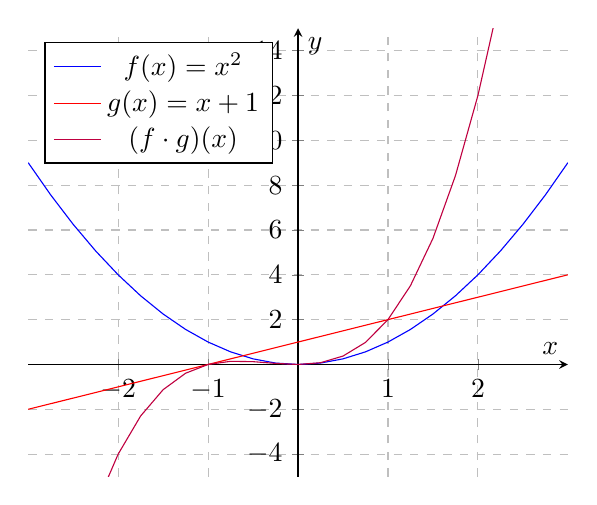
\begin{tikzpicture}
\begin{axis}[
    axis lines = middle,
    xlabel = $x$,
    ylabel = $y$,
    xmin = -3, xmax = 3,
    ymin = -5, ymax = 15,
    xtick = {-2,-1,0,1,2},
    ytick = {-4,-2,0,2,4,6,8,10,12,14},
    legend pos = north west,
    ymajorgrids = true,
    xmajorgrids = true,
    grid style = dashed,
]

\addplot[domain=-3:3, blue] {x^2};
\addlegendentry{$f(x) = x^2$}

\addplot[domain=-3:3, red] {x + 1};
\addlegendentry{$g(x) = x + 1$}

\addplot[domain=-3:3, purple] {x^2 * (x + 1)};
\addlegendentry{$(f \cdot g)(x)$}

\end{axis}
\end{tikzpicture}
\end{center}

\begin{center}
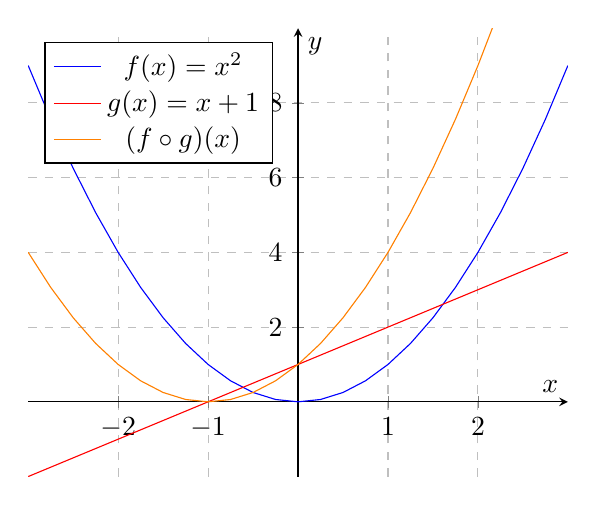
\begin{tikzpicture}
\begin{axis}[
    axis lines = middle,
    xlabel = $x$,
    ylabel = $y$,
    xmin = -3, xmax = 3,
    ymin = -2, ymax = 10,
    xtick = {-2,-1,0,1,2},
    ytick = {0,2,4,6,8},
    legend pos = north west,
    ymajorgrids = true,
    xmajorgrids = true,
    grid style = dashed,
]

\addplot[domain=-3:3, blue] {x^2};
\addlegendentry{$f(x) = x^2$}

\addplot[domain=-3:3, red] {x + 1};
\addlegendentry{$g(x) = x + 1$}

\addplot[domain=-3:3, orange] {(x + 1)^2};
\addlegendentry{$(f \circ g)(x)$}

\end{axis}
\end{tikzpicture}
\end{center}

\section{Inverse Functions}

An inverse function "undoes" what the original function does.

\subsection{Definition}

For a function $f$, its inverse function $f^{-1}$ satisfies:
\begin{itemize}
    \item $f(f^{-1}(x)) = x$
    \item $f^{-1}(f(x)) = x$
\end{itemize}

\subsection{Finding Inverse Functions}

To find the inverse of $y = f(x)$:
1. Replace $f(x)$ with $y$
2. Interchange $x$ and $y$
3. Solve for $y$
4. Replace $y$ with $f^{-1}(x)$

\subsection{Example 8: Finding an Inverse Function}

Find the inverse of $f(x) = 2x + 3$.

Solution:
1. $y = 2x + 3$
2. $x = 2y + 3$
3. $x - 3 = 2y$
   $\frac{x - 3}{2} = y$
4. $f^{-1}(x) = \frac{x - 3}{2}$

\subsection{Graphical Relationship}

The graph of $f^{-1}(x)$ is the reflection of $f(x)$ over the line $y = x$.

\begin{center}
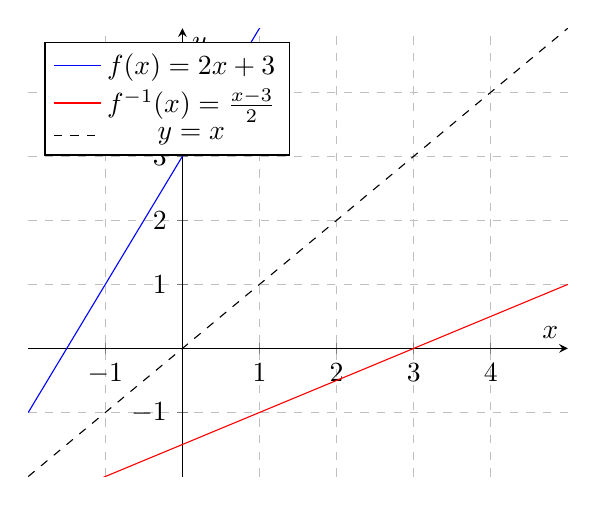
\begin{tikzpicture}
\begin{axis}[
    axis lines = middle,
    xlabel = $x$,
    ylabel = $y$,
    xmin = -2, xmax = 5,
    ymin = -2, ymax = 5,
    xtick = {-1,0,1,2,3,4},
    ytick = {-1,0,1,2,3,4},
    legend pos = north west,
    ymajorgrids = true,
    xmajorgrids = true,
    grid style = dashed,
]

\addplot[domain=-2:5, blue] {2*x + 3};
\addlegendentry{$f(x) = 2x + 3$}

\addplot[domain=-2:5, red] {(x-3)/2};
\addlegendentry{$f^{-1}(x) = \frac{x-3}{2}$}

\addplot[domain=-2:5, dashed] {x};
\addlegendentry{$y = x$}

\end{axis}
\end{tikzpicture}
\end{center}

\subsection{More Examples of Inverse Functions}

Let's look at some other common functions and their inverses.

\subsubsection{Square Function and Square Root Function}

$f(x) = x^2$ (for $x \geq 0$) and its inverse $f^{-1}(x) = \sqrt{x}$

\begin{center}
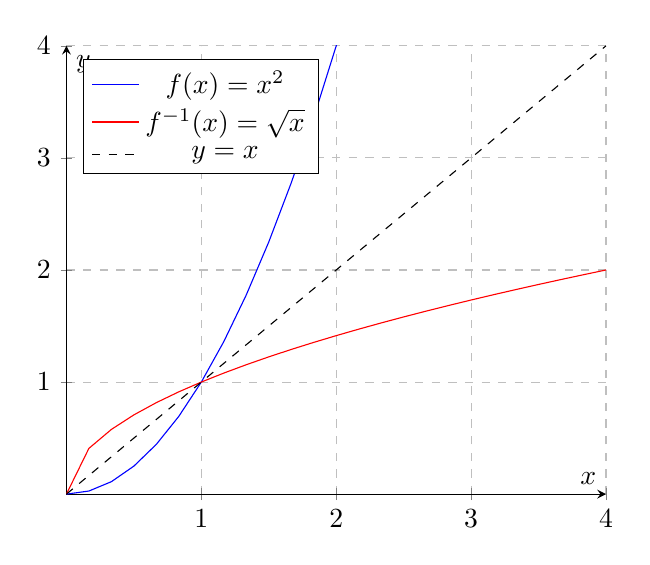
\begin{tikzpicture}
\begin{axis}[
    axis lines = middle,
    xlabel = $x$,
    ylabel = $y$,
    xmin = 0, xmax = 4,
    ymin = 0, ymax = 4,
    xtick = {1,2,3,4},
    ytick = {1,2,3,4},
    legend pos = north west,
    ymajorgrids = true,
    xmajorgrids = true,
    grid style = dashed,
]

\addplot[domain=0:4, blue] {x^2};
\addlegendentry{$f(x) = x^2$}

\addplot[domain=0:4, red] {sqrt(x)};
\addlegendentry{$f^{-1}(x) = \sqrt{x}$}

\addplot[domain=0:4, dashed] {x};
\addlegendentry{$y = x$}

\end{axis}
\end{tikzpicture}
\end{center}

Note: We restrict the domain of $f(x) = x^2$ to non-negative numbers to ensure it has an inverse.

\subsubsection{Exponential and Logarithmic Functions}

$f(x) = 2^x$ and its inverse $f^{-1}(x) = \log_2(x)$

\begin{center}
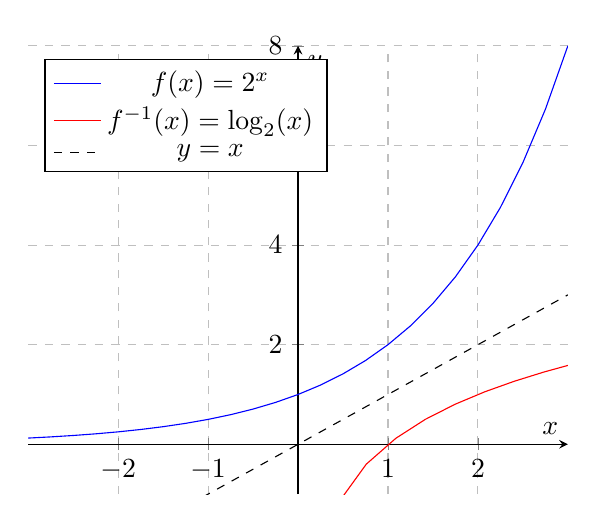
\begin{tikzpicture}
\begin{axis}[
    axis lines = middle,
    xlabel = $x$,
    ylabel = $y$,
    xmin = -3, xmax = 3,
    ymin = -1, ymax = 8,
    xtick = {-2,-1,0,1,2},
    ytick = {0,2,4,6,8},
    legend pos = north west,
    ymajorgrids = true,
    xmajorgrids = true,
    grid style = dashed,
]

\addplot[domain=-3:3, blue] {2^x};
\addlegendentry{$f(x) = 2^x$}

\addplot[domain=0.1:8, red] {log2(x)};
\addlegendentry{$f^{-1}(x) = \log_2(x)$}

\addplot[domain=-3:3, dashed] {x};
\addlegendentry{$y = x$}

\end{axis}
\end{tikzpicture}
\end{center}

\newpage
\subsection{Properties of Inverse Function Graphs}

1. The graphs of a function and its inverse are symmetric about the line $y = x$.
2. If $(a, b)$ is a point on the graph of $f$, then $(b, a)$ is a point on the graph of $f^{-1}$.
3. The domain of $f$ becomes the range of $f^{-1}$, and vice versa.
4. Not all functions have inverses. To have an inverse, a function must be one-to-one (injective).

\subsection{One-to-One Functions}

A function is one-to-one if each element of the codomain is paired with at most one element of the domain. Graphically, this means that no horizontal line intersects the graph of the function more than once.

\begin{center}
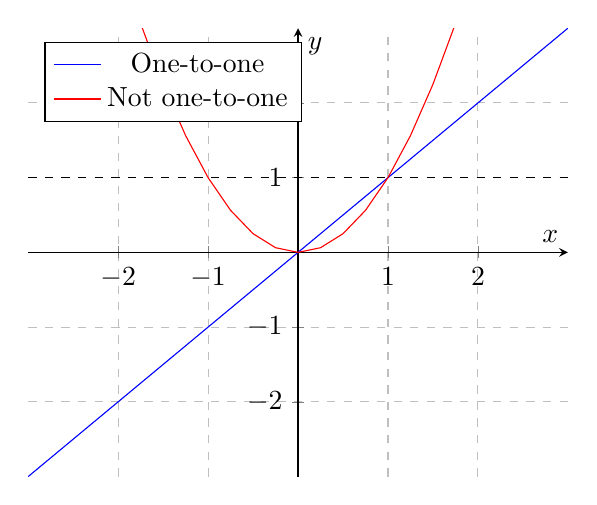
\begin{tikzpicture}
\begin{axis}[
    axis lines = middle,
    xlabel = $x$,
    ylabel = $y$,
    xmin = -3, xmax = 3,
    ymin = -3, ymax = 3,
    xtick = {-2,-1,0,1,2},
    ytick = {-2,-1,0,1,2},
    legend pos = north west,
    ymajorgrids = true,
    xmajorgrids = true,
    grid style = dashed,
]

\addplot[domain=-3:3, blue] {x};
\addlegendentry{One-to-one}

\addplot[domain=-3:3, red] {x^2};
\addlegendentry{Not one-to-one}

\draw[dashed] (-3,1) -- (3,1);
\node[anchor=west] at (axis cs: 3,1) {$y = 1$};

\end{axis}
\end{tikzpicture}
\end{center}

\section{Practice Problems}

\subsection{Problem 1: Function Composition}

Let $f(x) = x + 2$ and $g(x) = x^2$.

a) Find $(f \circ g)(x)$.

b) Find $(g \circ f)(x)$.

c) Evaluate $(f \circ g)(3)$.

\vspace{2cm}
Answer:
\vspace{3cm}

\subsection{Problem 2: Function Transformations}

Starting with the function $f(x) = |x|$, graph $g(x) = |x - 2| + 3$.

Describe the transformations applied to $f(x)$ to get $g(x)$.

\vspace{2cm}
Answer:
\vspace{2cm}

\begin{center}
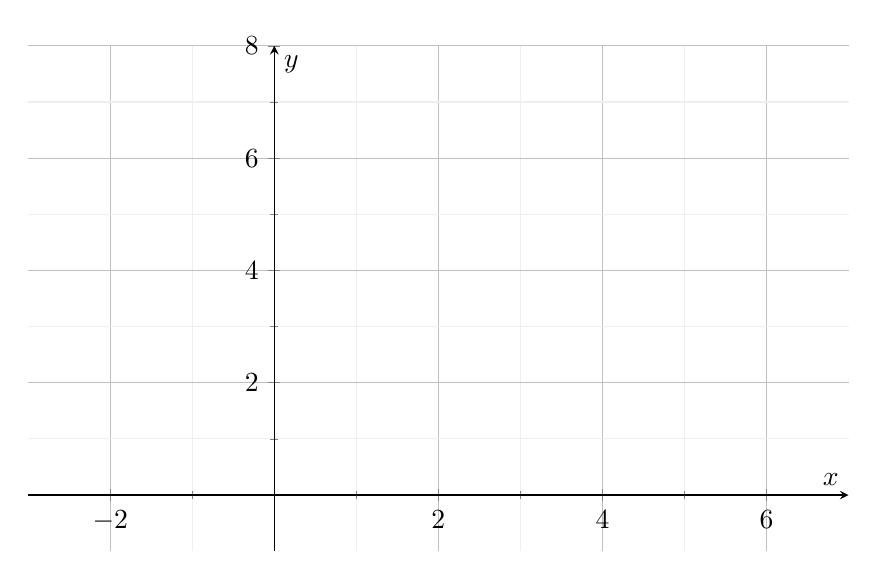
\begin{tikzpicture}
\begin{axis}[
    axis lines = middle,
    xlabel = $x$,
    ylabel = $y$,
    xmin = -3, xmax = 7,
    ymin = -1, ymax = 8,
    xtick = {-2,0,2,4,6},
    ytick = {0,2,4,6,8},
    grid = both,
    minor tick num = 1,
    major grid style = {lightgray},
    minor grid style = {lightgray!25},
    width = 12cm,
    height = 8cm,
]
\end{axis}
\end{tikzpicture}
\end{center}

\subsection{Problem 3: Combining Functions}

Let $f(x) = x + 1$ and $g(x) = x^2 - 4$.

a) Find an expression for $(f + g)(x)$.

b) Find an expression for $(f \cdot g)(x)$.

c) Evaluate $(f + g)(3)$ and $(f \cdot g)(3)$.

\vspace{2cm}
Answer:
\vspace{3cm}

\subsection{Problem 4: Inverse Functions}

Find the inverse function for $f(x) = 2x + 5$.

Then, find $f^{-1}(11)$.

\vspace{2cm}
Answer:
\vspace{3cm}

\subsection{Problem 5: Graphing Functions}

Graph the function $h(x) = x^2 - 4x + 3$.

a) Find the y-intercept.

b) Find the x-intercepts.

c) Find the vertex of the parabola.

d) Is the parabola opening upward or downward?

\vspace{2cm}
Answer:
\vspace{2cm}

\begin{center}
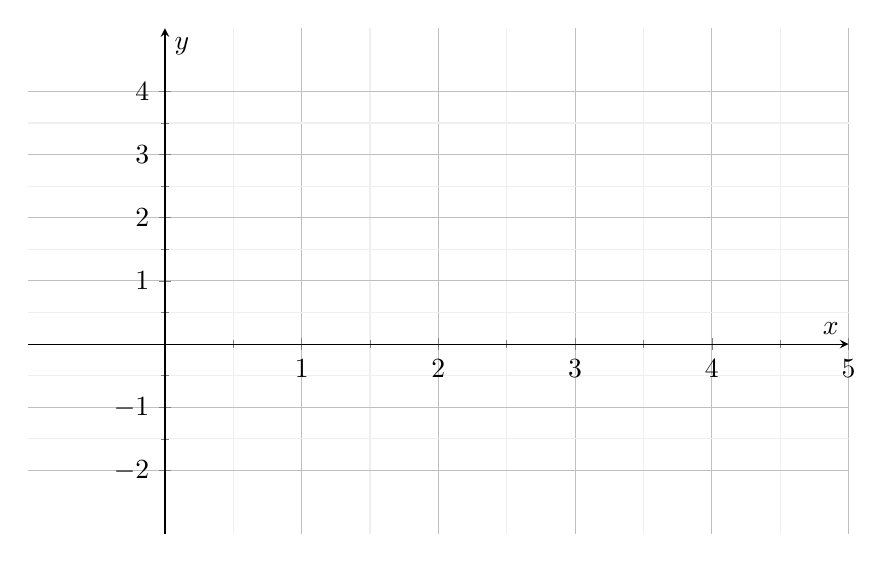
\begin{tikzpicture}
\begin{axis}[
    axis lines = middle,
    xlabel = $x$,
    ylabel = $y$,
    xmin = -1, xmax = 5,
    ymin = -3, ymax = 5,
    xtick = {0,1,2,3,4,5},
    ytick = {-2,-1,0,1,2,3,4},
    grid = both,
    minor tick num = 1,
    major grid style = {lightgray},
    minor grid style = {lightgray!25},
    width = 12cm,
    height = 8cm,
]
\end{axis}
\end{tikzpicture}
\end{center}

\subsection{Problem 6: Function Domain and Range}

For the function $f(x) = \sqrt{x - 1}$:

a) Find the domain of $f(x)$.

b) Find the range of $f(x)$.

c) Graph the function.

\vspace{2cm}
Answer:
\vspace{2cm}

\begin{center}
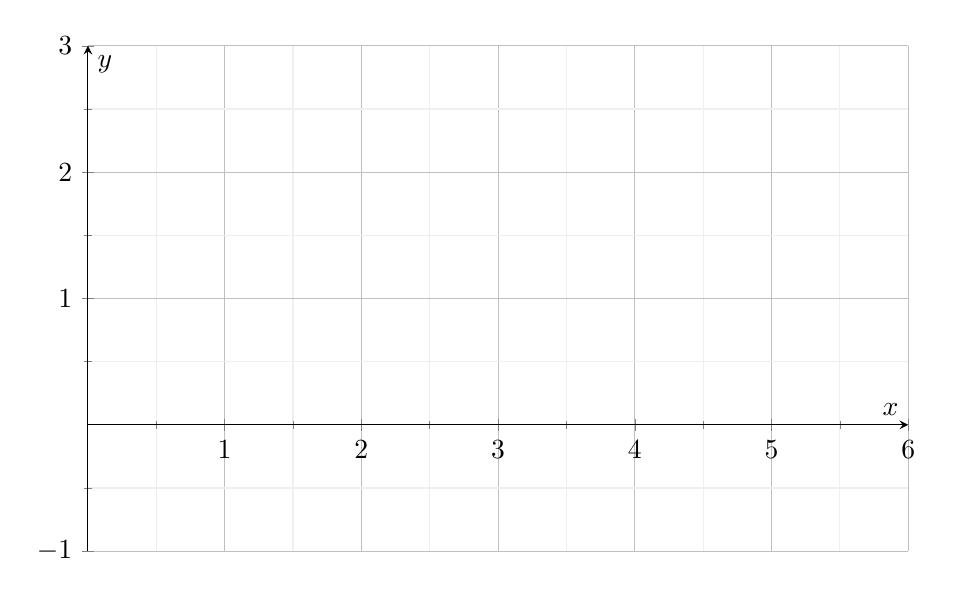
\begin{tikzpicture}
\begin{axis}[
    axis lines = middle,
    xlabel = $x$,
    ylabel = $y$,
    xmin = 0, xmax = 6,
    ymin = -1, ymax = 3,
    xtick = {0,1,2,3,4,5,6},
    ytick = {-1,0,1,2,3},
    grid = both,
    minor tick num = 1,
    major grid style = {lightgray},
    minor grid style = {lightgray!25},
    width = 12cm,
    height = 8cm,
]
\end{axis}
\end{tikzpicture}
\end{center}

\newpage

\section{Solutions to Practice Problems}

\subsection{Solution 1: Function Composition}

Let $f(x) = x + 2$ and $g(x) = x^2$.

a) $(f \circ g)(x) = f(g(x)) = g(x) + 2 = x^2 + 2$

b) $(g \circ f)(x) = g(f(x)) = (x + 2)^2 = x^2 + 4x + 4$

c) $(f \circ g)(3) = f(g(3)) = f(3^2) = f(9) = 9 + 2 = 11$

\subsection{Solution 2: Function Transformations}

Starting with $f(x) = |x|$, to get $g(x) = |x - 2| + 3$:

1. Shift 2 units right: $|x - 2|$
2. Shift 3 units up: $|x - 2| + 3$

Graph:

\begin{center}
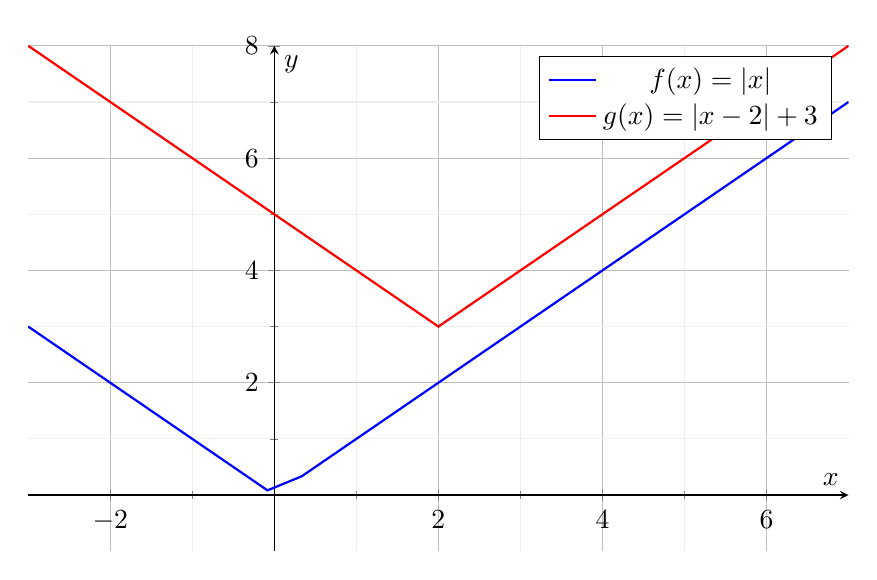
\begin{tikzpicture}
\begin{axis}[
    axis lines = middle,
    xlabel = $x$,
    ylabel = $y$,
    xmin = -3, xmax = 7,
    ymin = -1, ymax = 8,
    xtick = {-2,0,2,4,6},
    ytick = {0,2,4,6,8},
    grid = both,
    minor tick num = 1,
    major grid style = {lightgray},
    minor grid style = {lightgray!25},
    width = 12cm,
    height = 8cm,
]
\addplot[blue, thick, domain=-3:7] {abs(x)};
\addplot[red, thick, domain=-3:7] {abs(x-2)+3};
\legend{$f(x) = |x|$, $g(x) = |x-2|+3$}
\end{axis}
\end{tikzpicture}
\end{center}

\subsection{Solution 3: Combining Functions}

Let $f(x) = x + 1$ and $g(x) = x^2 - 4$.

a) $(f + g)(x) = f(x) + g(x) = (x + 1) + (x^2 - 4) = x^2 + x - 3$

b) $(f \cdot g)(x) = f(x) \cdot g(x) = (x + 1)(x^2 - 4)$

c) $(f + g)(3) = 3^2 + 3 - 3 = 9 + 3 - 3 = 9$
   $(f \cdot g)(3) = (3 + 1)(3^2 - 4) = 4(9 - 4) = 4(5) = 20$

\subsection{Solution 4: Inverse Functions}

For $f(x) = 2x + 5$:

1. Replace $f(x)$ with $y$: $y = 2x + 5$
2. Swap $x$ and $y$: $x = 2y + 5$
3. Solve for $y$: 
   $x - 5 = 2y$
   $\frac{x - 5}{2} = y$

Therefore, $f^{-1}(x) = \frac{x - 5}{2}$

To find $f^{-1}(11)$:
$f^{-1}(11) = \frac{11 - 5}{2} = \frac{6}{2} = 3$

\subsection{Solution 5: Graphing Functions}

For $h(x) = x^2 - 4x + 3$:

a) Y-intercept: When $x = 0$, $y = 0^2 - 4(0) + 3 = 3$. So, the y-intercept is (0, 3).

b) X-intercepts: Solve $x^2 - 4x + 3 = 0$
   $(x - 1)(x - 3) = 0$
   $x = 1$ or $x = 3$
   X-intercepts are (1, 0) and (3, 0).

c) Vertex: $x = -b/(2a) = -(-4)/(2(1)) = 2$
   $y = 2^2 - 4(2) + 3 = 4 - 8 + 3 = -1$
   Vertex is (2, -1).

d) The parabola opens upward because the coefficient of $x^2$ is positive.

Graph:

\begin{center}
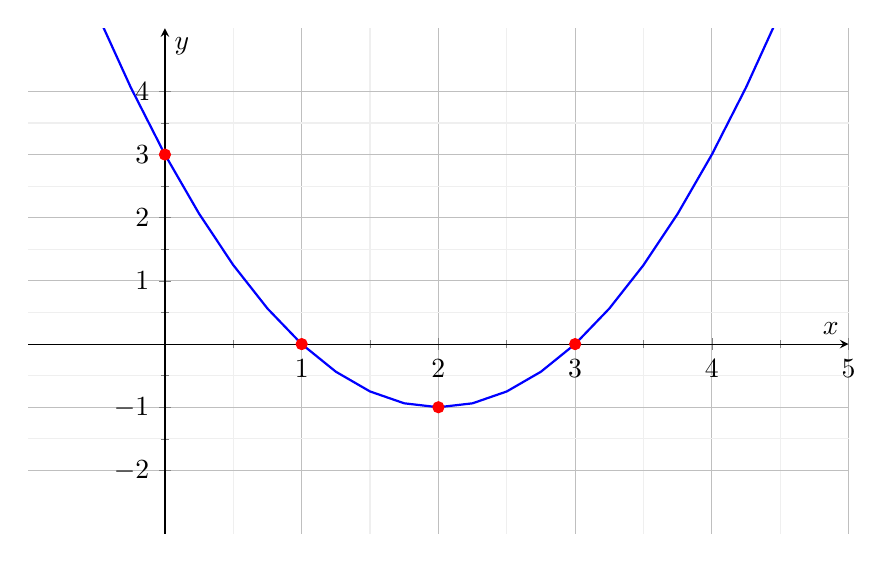
\begin{tikzpicture}
\begin{axis}[
    axis lines = middle,
    xlabel = $x$,
    ylabel = $y$,
    xmin = -1, xmax = 5,
    ymin = -3, ymax = 5,
    xtick = {0,1,2,3,4,5},
    ytick = {-2,-1,0,1,2,3,4},
    grid = both,
    minor tick num = 1,
    major grid style = {lightgray},
    minor grid style = {lightgray!25},
    width = 12cm,
    height = 8cm,
]
\addplot[blue, thick, domain=-1:5] {x^2 - 4*x + 3};
\addplot[only marks, red] coordinates {(0,3) (1,0) (3,0) (2,-1)};
\end{axis}
\end{tikzpicture}
\end{center}

\subsection{Solution 6: Function Domain and Range}

For $f(x) = \sqrt{x - 1}$:

a) Domain: The expression under the square root must be non-negative.
   $x - 1 \geq 0$
   $x \geq 1$
   Domain is $[1, \infty)$

b) Range: Since $\sqrt{x - 1} \geq 0$ for all $x$ in the domain, and there's no upper limit,
   Range is $[0, \infty)$

c) Graph:

\begin{center}
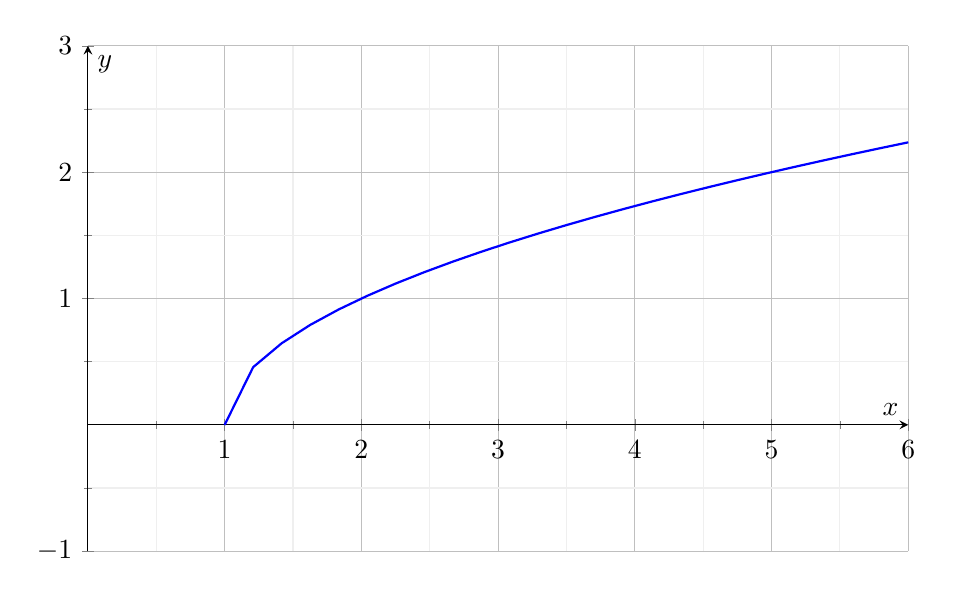
\begin{tikzpicture}
\begin{axis}[
    axis lines = middle,
    xlabel = $x$,
    ylabel = $y$,
    xmin = 0, xmax = 6,
    ymin = -1, ymax = 3,
    xtick = {0,1,2,3,4,5,6},
    ytick = {-1,0,1,2,3},
    grid = both,
    minor tick num = 1,
    major grid style = {lightgray},
    minor grid style = {lightgray!25},
    width = 12cm,
    height = 8cm,
]
\addplot[blue, thick, domain=1:6] {sqrt(x-1)};
\end{axis}
\end{tikzpicture}
\end{center}

\end{document}